\documentclass{ieeeaccess}
\usepackage{cite}
\usepackage{comment}
\usepackage{hyperref}
\hypersetup{
    colorlinks=true,
    linkcolor=blue,
    filecolor=blue,      
    urlcolor=blue,
    }

\usepackage{float}
\usepackage{svg}
\usepackage{amsmath}
\usepackage{amsmath,amssymb,amsfonts}
\usepackage{tikz}
 \NewSpotColorSpace{PANTONE}
  \AddSpotColor{PANTONE} {PANTONE3015C} {PANTONE\SpotSpace 3015\SpotSpace C} {1 0.3 0 0.2}
  \SetPageColorSpace{PANTONE}
\usetikzlibrary{shapes, arrows.meta, positioning}

\usepackage{algorithmic}
\usepackage{graphicx}
\usepackage{textcomp}
\def\BibTeX{{\rm B\kern-.05em{\sc i\kern-.025em b}\kern-.08em
    T\kern-.1667em\lower.7ex\hbox{E}\kern-.125emX}}

\usepackage{xcolor}
\usepackage{orcidlink}

\begin{document}
\history{Manuscript prepared on May 25, 2026.}
\doi{}

\title{A Unified Framework for Designing Swarm Robots Using a Model-Based Systems Engineering Approach
%: A Comprehensive Approach to Hardware, and Software
}
%\author{\uppercase{Hoang Anh Pham}
\author{\uppercase{Hoang Anh Pham}
\orcidlink{0000-0001-9621-9266}
\authorrefmark{1}, %\IEEEmembership{Fellow, IEEE},
%\uppercase{Thierry Soriano}\authorrefmark{1}, and \uppercase{Valentin Gies}\authorrefmark{2}, 
\uppercase{Valentin Gies}\authorrefmark{2}, and \uppercase{Thierry Soriano}\authorrefmark{3}, 
%and \uppercase{FULL Name}\authorrefmark{2}
%\IEEEmembership{Member, IEEE}
}

\address[1]{Faculty of Electronics Engineering 1, Post and Telecommunications Institute of Technology, Hanoi, Vietnam 
%(e-mail: author@boulder.nist.gov)
}

\address[2]{Laboratory IM2NP, University of Toulon, Toulon, France 
%(e-mail: author@lamar.colostate.edu)
}

\address[3]{Laboratory COSMER, University of Toulon, Toulon, France 
%(e-mail: author@boulder.nist.gov)
}
%\address[3]{Electrical Engineering Department, University of Colorado, Boulder, CO 80309 USA}
%\tfootnote{This work was supported by the French ANR/AID agency under the RoboSCo project}
%\tfootnote{This work was supported by the University of Toulon except Mr. Hoang Anh Pham}
\markboth
{Pham \headeretal: From SysML to ROS 2 for Two TurtleBot4 Robots}
{Pham \headeretal: From SysML to ROS 2 for Two TurtleBot4 Robots}

\corresp{Corresponding author: Hoang Anh Pham (e-mail: anhph@ptit.edu.vn).}
%\corresp{Corresponding author: Thierry Soriano (e-mail: thierry-soriano@univ-tln.fr).}


\begin{abstract}
Multi-robot applications are difficult to validate when system models, simulation assets, and robot software evolve separately. This paper presents a model-based systems engineering (MBSE) workflow that connects SysML artifacts to an executable ROS 2 implementation for a two-TurtleBot4 target-acquisition mission. The workflow defines requirements, behavioral views, software architecture, hardware architecture, and data-flow views, then maps them to ROS 2 nodes, topics, launch files, DDS network settings, and validation metrics. The implemented case study uses exactly two canonical robot identities, \texttt{/robot1} and \texttt{/robot2}, while the physical TurtleBot4 Lite deployment boundary records the required FastDDS, \texttt{ROS\_DOMAIN\_ID}, Simple Discovery, and \texttt{/cmd\_vel\_unstamped} interfaces. A coordinator assigns the closest robot with fresh odometry as attacker, assigns the second robot a support pose near the target, publishes observable task state and events, and records the result in CSV metrics. A stable Gazebo simulation with TurtleBot4 visual models validates the executable chain before physical deployment. The latest run completed the mission in 8.028 s with no role switches and a minimum inter-robot separation of 0.6985 m. The contribution is not a general swarm benchmark, but a traceable sim-to-real workflow whose scope is deliberately aligned with the available two-robot platform.
\end{abstract}

\begin{keywords}
Model-based systems engineering, SysML, TurtleBot4, ROS 2, swarm robots, sim-to-real validation
\end{keywords}

\titlepgskip=-21pt

\maketitle

\section{Introduction}
Model-based systems engineering (MBSE) is increasingly used to manage the interaction between requirements, architecture, behavior, and verification in complex engineered systems \cite{Sannes2022,Zihang2024}. Robotics brings the same integration problem into a smaller but more dynamic setting: the model must remain consistent with sensors, computation, communication, motion control, simulation, and hardware deployment. This consistency is especially important for multi-robot systems because a coordination error may be caused by an ambiguous requirement, an incomplete architecture model, a ROS 2 namespace or \texttt{ROS\_DOMAIN\_ID} mismatch, a simulator limitation, or a hardware safety constraint.

This paper studies that problem through a deliberately bounded case study: two TurtleBot4 robots performing a target-acquisition mission. One robot is assigned as the attacker and moves toward the target. The second robot is assigned as the supporter and moves to an offset pose near the same target. The number of robots is fixed by the available physical platform, and the paper does not claim validation beyond this two-robot setting.

The central research question is how to keep SysML models useful after the transition from conceptual design to executable ROS 2 code. Rather than treating SysML diagrams as documentation only, the proposed workflow uses them as traceability anchors for the implementation: requirements are mapped to nodes, topics, launch files, runtime events, DDS settings, and metrics. The same canonical robot identities are used in simulation and in the physical deployment adapter so that the design boundary is explicit.

The contributions of this paper are:
\begin{itemize}
    \item a SysML-based workflow that connects requirements, activity, structure, software architecture, hardware architecture, and data-flow views for a two-TurtleBot4 mission;
    \item a ROS 2 implementation that realizes the modeled behavior through \texttt{/robot1} and \texttt{/robot2} canonical identities, observable roles, target goals, task state, and metrics;
    \item a sim-to-real deployment boundary in which simulation is executable by default and physical motion commands require explicit enablement;
    \item an evaluation run showing that the modeled requirements can be traced to a completed simulation result.
\end{itemize}

The rest of the paper is organized as follows. Section II reviews related work on swarm robotics, MBSE, SysML, and ROS-based systems. Section III presents the proposed MBSE-to-ROS 2 workflow. Section IV describes the two-TurtleBot4 case study and validation results. Section V concludes the paper and identifies remaining limitations.

\section{Related Work}
\subsection{Swarm robotics and multi-robot coordination}
Swarm robotics studies how multiple robots can coordinate through task allocation, navigation, communication, and local decision-making. Surveys of swarm robotics tasks emphasize behaviors such as aggregation, flocking, foraging, deployment, collaborative manipulation, and task allocation \cite{Bayindir2016}. From a swarm engineering perspective, these behaviors must be designed, verified, and maintained through systematic processes rather than through isolated controller implementations \cite{Manuele2013}. Mission-oriented architectures for unmanned swarms further show that reusable mission structure is useful when the same coordination logic must be adapted to different platforms or scenarios \cite{Giles2019}.

The present work does not attempt to cover all swarm behaviors. It selects one representative coordination problem--role allocation for target acquisition--and uses it to demonstrate traceability from system requirements to executable ROS 2 behavior. This narrower scope makes the validation boundary explicit and keeps the experiment aligned with the available two-TurtleBot4 platform.

\subsection{MBSE and SysML for executable engineering}
MBSE replaces scattered document artifacts with linked models that capture requirements, structure, behavior, and verification intent \cite{Sannes2022,Zihang2024}. SysML has been used to structure engineering knowledge at multiple abstraction levels, allowing high-level decisions to remain connected to lower-level design elements \cite{Luca2011}. Systems-thinking work also emphasizes the transition from problem capture to formal SysML models, reducing information loss between early design and engineering artifacts \cite{Cloutier2015}.

Several domains have demonstrated the value of MBSE for architecture and traceability, including aircraft systems \cite{Li2019,Zhiyang2022}, satellite communication systems \cite{SuGao2019}, and digital twins for industrial robots \cite{Zhang2023}. These works show that MBSE is most useful when the model supports downstream analysis or implementation. The contribution here is to apply the same principle to a small mobile-robot team and to keep the SysML artifacts connected to concrete ROS 2 entities and measured simulation results.

\subsection{ROS-based robotic systems}
ROS and ROS 2 provide a practical middleware layer for robotic software, but the flexibility of nodes, topics, parameters, and launch files can make architecture-level consistency difficult to maintain. A SysML-based metamodel for ROS systems has been proposed to represent both runtime systems and developer workspaces \cite{Winiarski2023}. Supervisory controller synthesis for ROS-based applications also illustrates the need to connect requirements with executable robotic behavior \cite{S2023}. This paper follows the same motivation from a traceability perspective: every requirement in the case study is linked to a ROS 2 artifact and a runtime metric.

\begin{figure}[H]
  \centering 
  %\includegraphics[scale = 0.35]{figs/Simulation_1.png}
  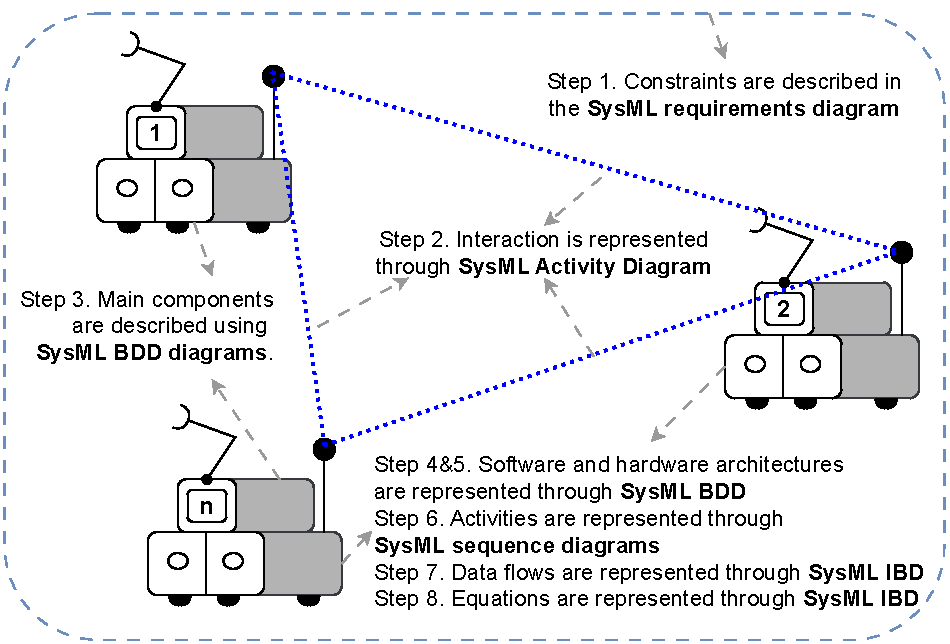
\includegraphics[scale = 0.525]{figs/Swarmrobot.pdf}
  \caption{Illustrating the use of SysML in the design of swarm robotics}
  \label{fig_SysML_Swarms}
\end{figure}

\subsection{SysML Framework for Swarm Robots}
The objective of using SysML is to provide a standardized method for modeling and integrating the hardware, software, and behavioral aspects of a coordinated robot team (see Figure \ref{fig_SysML_Swarms}). In this paper, the validated team contains two TurtleBot4 robots. The same modeling pattern can be reused for larger teams, but larger teams are outside the validation boundary of the present work.
\begin{itemize}
    \item \textbf{Modeling language:} SysML is used because it represents requirements, behavior, structure, and inter-component relationships within one consistent notation.
    \item \textbf{Tool independence:} The workflow does not depend on a specific SysML tool; it requires only support for requirement diagrams, block definition diagrams, activity diagrams, sequence diagrams, and internal block diagrams.
    \item \textbf{Modeling conventions:} Requirement identifiers, robot identities, ROS 2 topic names, DDS domain settings, and validation metrics are kept consistent so that each diagram can be traced to an executable artifact.
\end{itemize}

%\newpage
\section{Proposed MBSE-to-ROS 2 Workflow}
The proposed workflow links a SysML model to executable ROS 2 artifacts. It is organized around four questions: what must the two-robot system do, how is the mission behavior represented, which software and hardware elements realize the behavior, and how is the result verified. Figure \ref{fig_diagram_req} captures the top-level requirements, Figures \ref{fig_SwarmRoboticsTasks}--\ref{fig_diag_sque_2} provide behavioral and structural views, and Figures \ref{fig_bdd_software}--\ref{fig_IBD_DataFlow} connect the model to implementation and platform concerns.

\subsection{Requirement Model and Traceability}
The requirement model defines the validation boundary before implementation. The mission contains exactly two TurtleBot4 robots. They cooperate on one target-acquisition task, assign attacker and supporter roles from fresh odometry, publish observable state, validate the behavior in simulation before physical deployment, and preserve a documented mapping to the physical TurtleBot4 Lite network configuration. This early boundary is important because it prevents the model from implying a robot team size or capability that is not available in the experimental platform.

\begin{figure}[htbp]
  \centering
  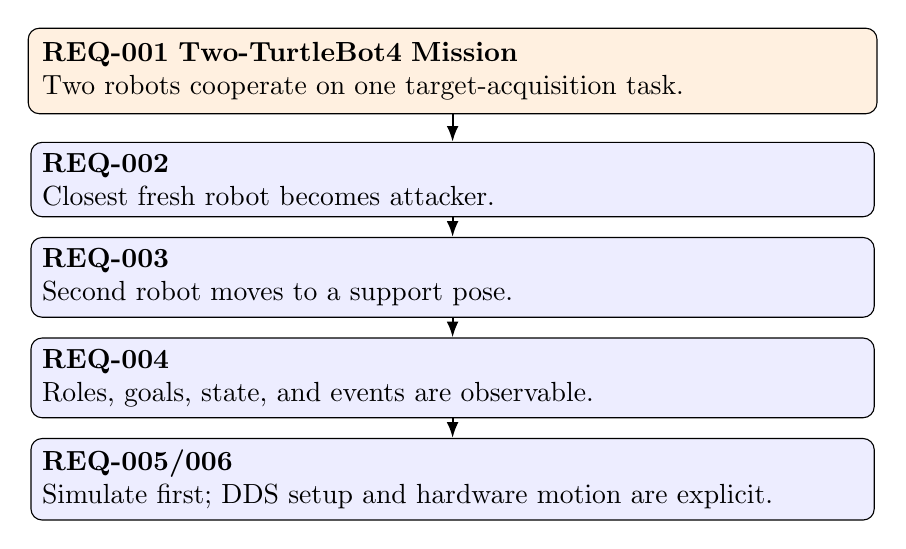
\begin{tikzpicture}[
    req/.style={draw, rounded corners, fill=orange!12, align=left, text width=0.86\columnwidth, inner sep=5pt},
    subreq/.style={draw, rounded corners, fill=blue!7, align=left, text width=0.86\columnwidth, inner sep=4pt},
    link/.style={-{Latex[length=2mm]}, thick}
  ]
    \node[req] (top) {\textbf{REQ-001 Two-TurtleBot4 Mission}\\Two robots cooperate on one target-acquisition task.};
    \node[subreq, below=0.35cm of top] (role) {\textbf{REQ-002}\\Closest fresh robot becomes attacker.};
    \node[subreq, below=0.25cm of role] (support) {\textbf{REQ-003}\\Second robot moves to a support pose.};
    \node[subreq, below=0.25cm of support] (obs) {\textbf{REQ-004}\\Roles, goals, state, and events are observable.};
    \node[subreq, below=0.25cm of obs] (val) {\textbf{REQ-005/006}\\Simulate first; DDS setup and hardware motion are explicit.};
    \draw[link] (top) -- (role);
    \draw[link] (role) -- (support);
    \draw[link] (support) -- (obs);
    \draw[link] (obs) -- (val);
  \end{tikzpicture}
  \caption{High-level requirements for the implemented two-TurtleBot4 case study}
  \label{fig_diagram_req}
\end{figure}

Each requirement is later mapped to a ROS 2 artifact: the coordinator node realizes role allocation, goal topics realize target and support assignments, launch files define simulation and physical modes, and CSV metrics provide evidence for verification. This gives the paper a traceable path from requirement to runtime result rather than a diagram-only model.

\subsection{Behavioral and Structural SysML Views}
The behavioral model uses a general swarm-task taxonomy as context, but selects task allocation, navigation, communication, and metric reporting as the executable subset for this study. Figure \ref{fig_SwarmRoboticsTasks} shows the broader task model, while Figure \ref{fig_Activity_Diagram} shows the activity pattern used by the mission: sense state, exchange information, allocate a role, execute the assigned action, and report completion.

\begin{figure}[H]
  \centering
  \includesvg[width=0.48\textwidth]{figs/00.SwarmRoboticsTasks.svg}
  \caption{Swarm robotics task model used to locate the implemented behavior}
  \label{fig_SwarmRoboticsTasks}
\end{figure}

\begin{figure*}[htbp]
  \centering
  \includesvg[width=0.85\textwidth]{figs/ActivitySwarmRobots.svg}
  \caption{Activity model for task allocation and coordinated execution}
  \label{fig_Activity_Diagram}
\end{figure*}

The structural view decomposes an individual robot into sensing, communication, control, and actuation responsibilities. In the TurtleBot4 implementation, these responsibilities map to odometry and sensor streams, ROS 2 communication, coordinator decisions, and velocity-command interfaces. Figure \ref{fig_DetailRobot} gives the block-level view, and Figures \ref{fig_diag_sque_1} and \ref{fig_diag_sque_2} show the interaction sequence used when a robot receives a task, senses its environment, executes a motion command, and reports status.

\begin{figure}[htbp]
  \centering
  \includesvg[width=0.48\textwidth]{figs/DetailSwarmRoboticsTasks.svg}
  \caption{Robot-level structural decomposition for sensing, control, communication, and actuation}
  \label{fig_DetailRobot}
\end{figure}

\begin{figure*}[htbp]
  \centering
  \includesvg[width=0.8\textwidth]{figs/Model.svg}
  \caption{Robot interaction sequence for task assignment and sensing}
  \label{fig_diag_sque_1}
\end{figure*}

\begin{figure*}[htbp]
  \centering
  \includesvg[width=0.8\textwidth]{figs/Robot_i.svg}
  \caption{Robot interaction sequence for execution, feedback, and status reporting}
  \label{fig_diag_sque_2}
\end{figure*}

\subsection{Software Architecture Mapping}
The software architecture is deliberately small enough to be executable and inspectable. The coordinator consumes target and odometry information, assigns roles, publishes goals, and emits task state. The simulation-only goal follower converts goals into velocity commands. The metrics logger subscribes to task state, events, and odometry to record validation data. In physical deployment, the coordinator and metrics nodes can run without commanding robot motion; direct velocity following is disabled unless explicitly enabled for controlled testing and mapped to the TurtleBot4 Lite \texttt{/cmd\_vel\_unstamped} interface.

\begin{figure*}[htbp]
  \centering
  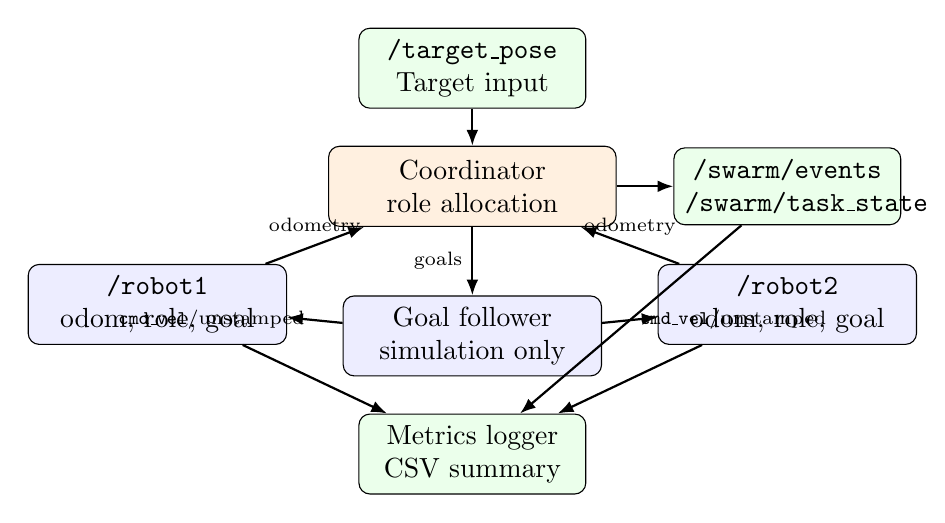
\begin{tikzpicture}[
    block/.style={draw, rounded corners, fill=blue!7, align=center, text width=3.0cm, minimum height=0.8cm, inner sep=4pt},
    core/.style={draw, rounded corners, fill=orange!12, align=center, text width=3.3cm, minimum height=0.9cm, inner sep=5pt},
    iface/.style={draw, rounded corners, fill=green!8, align=center, text width=2.6cm, minimum height=0.65cm, inner sep=4pt},
    arrow/.style={-{Latex[length=2mm]}, thick}
  ]
    \node[iface] (target) at (0,2.6) {\texttt{/target\_pose}\\Target input};
    \node[core] (coord) at (0,1.1) {Coordinator\\role allocation};
    \node[block] (r1) at (-4.0,-0.4) {\texttt{/robot1}\\odom, role, goal};
    \node[block] (r2) at (4.0,-0.4) {\texttt{/robot2}\\odom, role, goal};
    \node[block] (follower) at (0,-0.8) {Goal follower\\simulation only};
    \node[iface] (metrics) at (0,-2.3) {Metrics logger\\CSV summary};
    \node[iface] (events) at (4.0,1.1) {\texttt{/swarm/events}\\\texttt{/swarm/task\_state}};
    \draw[arrow] (target) -- (coord);
    \draw[arrow] (r1) -- node[above, font=\scriptsize] {odometry} (coord);
    \draw[arrow] (r2) -- node[above, font=\scriptsize] {odometry} (coord);
    \draw[arrow] (coord) -- node[left, font=\scriptsize] {goals} (follower);
    \draw[arrow] (follower) -- node[left, font=\scriptsize] {\texttt{cmd\_vel}/unstamped} (r1);
    \draw[arrow] (follower) -- node[right, font=\scriptsize] {\texttt{cmd\_vel}/unstamped} (r2);
    \draw[arrow] (coord) -- (events);
    \draw[arrow] (events) -- (metrics);
    \draw[arrow] (r1) -- (metrics);
    \draw[arrow] (r2) -- (metrics);
  \end{tikzpicture}
  \caption{Software architecture for the implemented two-TurtleBot4 mission}
  \label{fig_bdd_software}
\end{figure*}

The architecture in Figure \ref{fig_bdd_software} is mapped directly to the ROS 2 package. The \textbf{ControlSystem} is the \texttt{paper\_swarm\_coordinator} node. The \textbf{MissionState} is represented by \texttt{/target\_pose}, \texttt{/robot*/odom}, \texttt{/swarm/task\_state}, and \texttt{/swarm/events}. The \textbf{MotionControlModule} is represented by the goal follower in simulation and by the external navigation or safety stack when the physical robots are used. For TurtleBot4 Lite hardware, the command endpoint is treated as \texttt{/robot*/cmd\_vel\_unstamped} after namespace or bridge adaptation.

\subsection{Hardware and Data-Flow Views}
The hardware model identifies the platform assumptions that the software must respect: differential-drive motion, onboard computing, battery power, lidar/vision/IMU sensing, and wireless communication. The implementation uses TurtleBot4-class interfaces instead of a custom robot design, but the hardware view remains useful because it documents which physical resources are expected by the software architecture.

 \begin{figure*}[htbp]
  \centering
  \includesvg[width=1\textwidth]{figs/03.HardwareArchitecture.svg}
  \caption{Hardware architecture model for one TurtleBot4-class robot}
  \label{fig_HardwareArchitecture}
\end{figure*}

The Internal Block Diagram (IBD) in Figure \ref{fig_IBD_DataFlow} describes how data moves between sensing, processing, communication, power, and actuation elements. The corresponding software data-flow view in Figure \ref{fig_SoftwareDataFlow} connects those platform-level flows to the ROS 2 topics used by the mission. Together, the diagrams justify why odometry freshness, topic identities, DDS domain configuration, and command gating are treated as explicit requirements.

\begin{figure*}[htbp]
  \centering
  \includesvg[width=1\textwidth]{figs/ibd_RobotHardware.svg}
  \caption{Hardware data-flow model using an Internal Block Diagram}
  \label{fig_IBD_DataFlow}
\end{figure*}

\begin{figure*}[htbp]
  \centering
  \includesvg[width=1\textwidth]{figs/SoftwareFlowData.svg}
  \caption{Software data-flow view for one robot}
  \label{fig_SoftwareDataFlow}
\end{figure*}

%-------------------------------------------
%\newpage
\section{Case Study: Two TurtleBot4 Target Acquisition}
\subsection{Experimental Objective}
The case study evaluates whether the SysML requirements can be carried through to an executable ROS 2 mission without changing the system boundary. The experimental platform contains two TurtleBot4 robots, represented inside the model and simulator by the canonical identities \texttt{/robot1} and \texttt{/robot2}. A physical TurtleBot4 Lite, however, is commonly configured as a single robot with FastDDS, \texttt{ROS\_DOMAIN\_ID=0}, Simple Discovery, an empty user namespace, and root topics such as \texttt{/odom} and \texttt{/cmd\_vel\_unstamped} \cite{DuyTb4Lite2026,TurtleBot4Setup2026}. Therefore, a two-robot physical deployment must either assign unique namespaces in the shared ROS graph or bridge/remap two single-robot graphs into the canonical \texttt{/robot1} and \texttt{/robot2} interfaces. The mission is target acquisition: one robot moves to the target as attacker, while the other maintains a nearby support pose. This task is small, but it exercises the essential MBSE links used throughout the paper: requirement decomposition, role allocation, communication, software-to-hardware mapping, simulation validation, and physical deployment gating.

\begin{figure}[H]
  \centering
  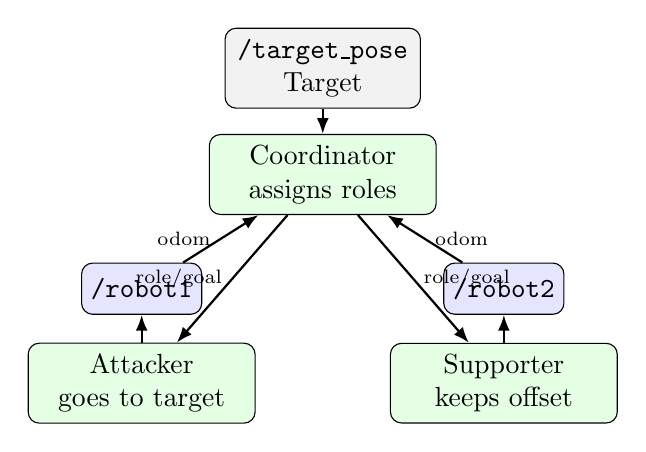
\begin{tikzpicture}[
    robot/.style={draw, rounded corners, fill=blue!10, minimum width=1.15cm, minimum height=0.65cm, align=center},
    role/.style={draw, rounded corners, fill=green!10, align=center, text width=2.6cm, inner sep=4pt},
    topic/.style={draw, rounded corners, fill=gray!10, align=center, text width=2.2cm, inner sep=4pt},
    arrow/.style={-{Latex[length=2mm]}, thick}
  ]
    \node[topic] (target) at (0,2.0) {\texttt{/target\_pose}\\Target};
    \node[role] (coord) at (0,0.65) {Coordinator\\assigns roles};
    \node[robot] (r1) at (-2.3,-0.8) {\texttt{/robot1}};
    \node[robot] (r2) at (2.3,-0.8) {\texttt{/robot2}};
    \node[role] (a) at (-2.3,-2.0) {Attacker\\goes to target};
    \node[role] (s) at (2.3,-2.0) {Supporter\\keeps offset};
    \draw[arrow] (target) -- (coord);
    \draw[arrow] (r1) -- node[left, font=\scriptsize] {odom} (coord);
    \draw[arrow] (r2) -- node[right, font=\scriptsize] {odom} (coord);
    \draw[arrow] (coord) -- node[left, font=\scriptsize] {role/goal} (a);
    \draw[arrow] (coord) -- node[right, font=\scriptsize] {role/goal} (s);
    \draw[arrow] (a) -- (r1);
    \draw[arrow] (s) -- (r2);
  \end{tikzpicture}
  \caption{Implemented two-TurtleBot4 attacker/supporter target-acquisition scenario}
  \label{fig_two_tb4_case}
\end{figure}

\subsection{Role Allocation Logic}
Let $p_T$ be the target position and $p_i$ be the latest odometry position for robot $i \in \{1,2\}$. A robot is eligible only if its odometry age $\Delta t_i$ is below the freshness threshold $\tau_{\max}$. The attacker is selected as
\[
    a=\arg\min_{i \in \{1,2\},\ \Delta t_i \le \tau_{\max}} \left\|p_i-p_T\right\|_2 .
\]
The other robot becomes the supporter. The attacker goal is the target itself, while the supporter goal is offset from the target:
\[
    g_a=p_T,\qquad
    g_s=p_T+\begin{bmatrix}d_x\\d_y\end{bmatrix}.
\]
A hysteresis margin is used to avoid unstable role switching when both robots are at similar distances from the target. This logic directly implements REQ-002 and REQ-003.

\subsection{Runtime Sequence}
The runtime sequence follows the activity model in Section III and is limited to target acquisition, role allocation, support positioning, and metric logging:
\begin{enumerate}
    \item A target is published on \texttt{/target\_pose}.
    \item Both TurtleBot4 robots publish fresh odometry on the canonical interfaces \texttt{/robot1/odom} and \texttt{/robot2/odom}, either directly through namespaces or through a physical remapping layer.
    \item The coordinator estimates distance from each robot to the target.
    \item The closest fresh robot becomes attacker, with a hysteresis margin to avoid unstable role switching.
    \item The second robot becomes supporter and receives a support goal offset from the target.
    \item Runtime state and events are published for debugging, traceability, and metric logging.
    \item Metrics are written to CSV files for validation and regression checks.
\end{enumerate}

\subsection{Traceability to ROS 2 Code}
The SysML requirements are implemented in the \texttt{paper\_tb4\_swarm} ROS 2 package. Table \ref{tab_traceability} summarizes the traceability link from each requirement to the executable artifact used in the case study.

\begin{table}[H]
\caption{Traceability between paper requirements and implementation}
\label{tab_traceability}
\centering
\begin{tabular}{p{0.18\columnwidth}p{0.36\columnwidth}p{0.34\columnwidth}}
\hline
\textbf{Req.} & \textbf{Design intent} & \textbf{Implementation} \\
\hline
REQ-001 & Two robots cooperate on one target task & \texttt{mbse\_model.py}, \texttt{coordinator.py} \\
REQ-002 & Closest fresh robot becomes attacker & \texttt{coordinator.py} role selection \\
REQ-003 & Second robot supports near target & \texttt{support\_offset\_x/y} parameters \\
REQ-004 & Roles, goals, states, events are observable & \texttt{/robot*/assigned\_role}, \texttt{/robot*/goal\_pose}, \texttt{/swarm/*} \\
REQ-005 & Simulation before hardware & \texttt{stable\_two\_tb4.launch.py}, CSV metrics \\
REQ-006 & Physical DDS setup and motion require explicit enablement & \texttt{real\_two\_tb4.launch.py}, \texttt{ROS\_DOMAIN\_ID}, \texttt{/cmd\_vel\_unstamped} \\
\hline
\end{tabular}
\end{table}

\subsection{Simulation and Physical Deployment Modes}
Two simulation modes are provided. The stable mode uses lightweight differential-drive physics with TurtleBot4 visual meshes. This mode is the preferred validation path on the current machine because full Gazebo rendering with the official TurtleBot4 stack previously crashed in the renderer. The official mode launches the installed TurtleBot4 simulator twice and is kept server-only by default.

The physical mode does not launch Gazebo and does not command TurtleBot4 motion by default. It starts the coordinator and metrics nodes against the canonical \texttt{/robot1} and \texttt{/robot2} interfaces. The lab baseline for each TurtleBot4 Lite is FastDDS with \texttt{ROS\_DOMAIN\_ID=0}, Simple Discovery, and no user namespace; in that single-robot form, the robot exposes root topics such as \texttt{/odom}, \texttt{/scan}, \texttt{/oakd/rgb/preview/image\_raw}, and \texttt{/cmd\_vel\_unstamped}. Two physical robots cannot both remain unnamespaced in the same ROS graph without topic collisions, so the deployment must either configure unique namespaces or provide an explicit bridge/remap layer before running the two-robot coordinator. Direct velocity following can be enabled only by setting an explicit launch argument during controlled lab testing, and the physical command topic is \texttt{/robot*/cmd\_vel\_unstamped}. This separation is intentional: the paper validates the model-to-code chain in simulation while preserving a conservative path for physical experiments.

\subsection{Simulation Result}
A stable simulation run was executed with the two TurtleBot4 namespaces and the attacker/supporter mission. The latest checked run produced the summary shown in Table \ref{tab_results}. The result validates the executable chain for target publication, odometry ingestion, role assignment, goal publication, robot motion, task completion, and metric logging.

\begin{table}[H]
\caption{Stable two-TurtleBot4 simulation result}
\label{tab_results}
\centering
\begin{tabular}{p{0.45\columnwidth}p{0.35\columnwidth}}
\hline
\textbf{Metric} & \textbf{Value} \\
\hline
Success & 1 \\
Duration & 8.028 s \\
Role switches & 0 \\
Minimum separation & 0.6985 m \\
\texttt{/robot1} path & 1.3808 m \\
\texttt{/robot2} path & 0.7805 m \\
Requirement refs & REQ-001--REQ-006 \\
\hline
\end{tabular}
\end{table}

\subsection{Discussion}
The result supports the paper's central claim: the same mission boundary defined in SysML is executable in ROS 2 and produces measurable validation evidence. The zero role-switch count indicates that the hysteresis margin prevented unnecessary reassignment during this run. The minimum separation remained positive, and both robot path lengths were recorded, confirming that the metrics logger observed the team-level behavior required by REQ-004.

The result should be interpreted within its intended scope. The simulation validates the traceability chain and the two-robot coordination behavior; it does not yet prove robustness across many environments, nor does it replace physical safety validation. For this reason, the physical launch mode keeps direct motion disabled unless the operator explicitly enables it.

\section{Conclusion and Discussion}
This paper presented a SysML-to-ROS 2 workflow for a two-TurtleBot4 target-acquisition mission. The workflow connects requirement, behavioral, structural, software, hardware, and data-flow models to executable ROS 2 nodes, topics, launch files, DDS settings, and metrics. The implemented case study assigns attacker and supporter roles from fresh odometry, publishes observable mission state, runs in simulation, and preserves the canonical \texttt{/robot1} and \texttt{/robot2} interfaces that can be connected to physical TurtleBot4 Lite robots through namespace or bridge adaptation.

The main limitation is that validation remains limited to a two-robot target-acquisition task and to the stable simulation mode. Future work will connect the physical TurtleBot4 robots through the real launch mode, replace the simple simulation follower with a safety-aware navigation stack, and evaluate the same traceability process across repeated trials and more varied environments.


%\section*{References}
%\begin{thebibliography}{00}
\bibliographystyle{ieeetr}
\bibliography{refs} % citation records are in the references.bib document
%\end{thebibliography}

%\section{Appendices}
%\begin{itemize}
%    \item Include additional material that supports the paper, such as detailed SysML diagrams, simulation data, or code snippets used in the project.
%\end{itemize}



%\appendices


%\section*{Acknowledgment}
%The preferred spelling of the word ``acknowledgment'' in American English is without an ``e'' after the ``g.'' Use the singular heading even if you have many acknowledgments. Avoid expressions such as ``One of us (S.B.A.) would like to thank $\ldots$ .'' Instead, write ``F. A. Author thanks $\ldots$ .'' In most cases, sponsor and financial support acknowledgments are placed in the unnumbered footnote on the first page, not here.


% Author biographies are omitted in this manuscript draft.
\EOD
\end{document}
